\documentclass[a4paper,10pt]{article}
\usepackage[margin=2.5cm]{geometry}

\usepackage{amssymb,amsmath,amsthm}
\usepackage{color}
\usepackage{enumitem}
\usepackage{dsfont}
\usepackage{bm}


\newtheorem{theorem}{Theorem}
\newtheorem{proposition}{Proposition}
\newtheorem{cor}{Corollary}
\theoremstyle{definition}
\newtheorem{definition}{Definition}
\newtheorem{remark}{Remark}
\newtheorem{example}{Example}
\newtheorem{claim}{Claim}
\newtheorem{lemma}{Lemma}


\usepackage{times} % use Times

\usepackage{../sty/shortcuts_js} % possibly adapted from https://github.com/josephsalmon/OrganizationFiles/sty/shortcuts_js.sty

%%%%%%%%%%%%%%%%%%%%%%%%%%%%%%%%%%%%%%%%%%%%%%%%%%%%%%%%%%%%%%%%%%%%%%%%%%%%%%%
% IMAGES
%%%%%%%%%%%%%%%%%%%%%%%%%%%%%%%%%%%%%%%%%%%%%%%%%%%%%%%%%%%%%%%%%%%%%%%%%%%%%%%

% Use prebuiltimages/ for images extracted from code (e.g. python)
% or to share images built from a software not available by the whole team (say matlab .fig, or inskcape .svg).
% .svg files should be stored in dir srcimages/ and built from moosetex if needed:
% https://www.charles-deledalle.fr/pages/moosetex.php
% NEVER (GIT) versions files in images/ : only prebuiltimages/ & srcimages/ !

\usepackage{graphicx} % For figures
\graphicspath{{images/}, {prebuiltimages/}}
\usepackage{subcaption}

%%%%%%%%%%%%%%%%%%%%%%%%%%%%%%%%%%%%%%%%%%%%%%%%%%%%%%%%%%%%%%%%%%%%%%%%%%%%%%%
% Algorithms
%%%%%%%%%%%%%%%%%%%%%%%%%%%%%%%%%%%%%%%%%%%%%%%%%%%%%%%%%%%%%%%%%%%%%%%%%%%%%%%

\usepackage{algorithm}
\usepackage[noend]{algorithmic}
\usepackage{hyperref}
\newcommand{\theHalgorithm}{\arabic{algorithm}}

%%%%%%%%%%%%%%%%%%%%%%%%%%%%%%%%%%%%%%%%%%%%%%%%%%%%%%%%%%%%%%%%%%%%%%%%%%%%%%%
% For citations
%%%%%%%%%%%%%%%%%%%%%%%%%%%%%%%%%%%%%%%%%%%%%%%%%%%%%%%%%%%%%%%%%%%%%%%%%%%%%%%

\usepackage[authoryear]{natbib}
\usepackage{cleveref} % mandatory for no pbs with hyperlinks theorem etc...
\crefformat{equation}{Eq.~(#2#1#3)} % format for equations
\Crefformat{equation}{Equation~(#2#1#3)} % format for equations


%%%%%%%%%%%%%%%%%%%%%%%%%%%%%%%%%%%%%%%%%%%%%%%%%%%%%%%%%%%%%%%%%%%%%%%%%%%%%%%
% Header and document start
%%%%%%%%%%%%%%%%%%%%%%%%%%%%%%%%%%%%%%%%%%%%%%%%%%%%%%%%%%%%%%%%%%%%%%%%%%%%%%%


\author{Joseph Salmon}
\title{Privacy preserving Lasso etc.}

\begin{document}

\maketitle

\vskip 0.3in

\begin{abstract}
This abstract is written here.
blabla.

\end{abstract}


%%%%%%%%%%%%%%%%%%%%%%%%%%%%%%%%%%%%%%%%%%%%%%%%%%%%%%%%%%%%%%%%%%%%%%%%%%%%%%%
% Sections in separated files
%%%%%%%%%%%%%%%%%%%%%%%%%%%%%%%%%%%%%%%%%%%%%%%%%%%%%%%%%%%%%%%%%%%%%%%%%%%%%%%

%!TEX root = ../article.tex


%%%%%%%%%%%%%%%%%%%%%%%%%%%%%%%%%%%%%%%%%%%%%%%%%%%%%%%%%%%%%%%%%%%%%%%%%%%%%%%
%%%%%%%%%%%%%%%%%%%%%%%%%%%%%%%%%%%%%%%%%%%%%%%%%%%%%%%%%%%%%%%%%%%%%%%%%%%%%%%
\section{Introduction}
\label{sec:introduction}
%%%%%%%%%%%%%%%%%%%%%%%%%%%%%%%%%%%%%%%%%%%%%%%%%%%%%%%%%%%%%%%%%%%%%%%%%%%%%%%
%%%%%%%%%%%%%%%%%%%%%%%%%%%%%%%%%%%%%%%%%%%%%%%%%%%%%%%%%%%%%%%%%%%%%%%%%%%%%%%

Let us remind first the famous Pythagoras' theorem:

\begin{align}\label{eq:pythagore}
	\norm{x+y}^2 = \norm{x}^2 + \norm{y}^2 \enspace.
\end{align}

Note that \Cref{eq:pythagore} is ok only under some conditions.
In terms of visualisation, you can reference a figure easily using the command \Cref{fig:pythagore} or using Fig.~\ref{fig:pythagore}.

\begin{figure}[h] % h stands for here
	\centering
	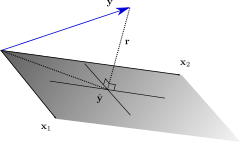
\includegraphics[width=0.6\textwidth]{residu_orth}
	\caption{Illustration of the residual orthogonality in least-squares.}
	\label{fig:pythagore}
\end{figure}


Also an image that is in the \texttt{prebuiltimages/} directory can also be loaded the same way:

\begin{figure}[h] % h stands for here, ! forces even more...
	\centering
	\includegraphics[width=0.2\textwidth]{umontpellier_logo}
	\caption{Illustration of a prebuiltimage available.}
	\label{fig:umontpellier_logo}
\end{figure}


For displaying side by side some images one should consider the package \lstinline+subcaptions+, that can be loaded with the \LaTeX command:

\begin{lstlisting}[language=tex]
\usepackage{subcaption}
\end{lstlisting}


\begin{figure}[t] % t stands for top (up!)
    \centering
    \begin{subfigure}[b]{0.33\textwidth}
    	\centering
        \includegraphics[width=0.2\textwidth]{umontpellier_logo}%
        \caption{First example}
        \label{subfig:pythagore}
    \end{subfigure}
    \begin{subfigure}[b]{0.56\textwidth}
    	\centering
        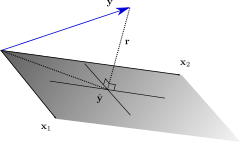
\includegraphics[width=0.5\textwidth]{residu_orth}%
        \caption{Second example}
        \label{subfig:logo}
    \end{subfigure}
    \caption{Exemples of side by side images}
    \label{fig:double_example}
\end{figure}


% ...more text here.
%!TEX root = ../main.tex


%%%%%%%%%%%%%%%%%%%%%%%%%%%%%%%%%%%%%%%%%%%%%%%%%%%%%%%%%%%%%%%%%%%%%%%%%%%%%%%
%%%%%%%%%%%%%%%%%%%%%%%%%%%%%%%%%%%%%%%%%%%%%%%%%%%%%%%%%%%%%%%%%%%%%%%%%%%%%%%
\section{Algorithms}
\label{sec:algorithms}
%%%%%%%%%%%%%%%%%%%%%%%%%%%%%%%%%%%%%%%%%%%%%%%%%%%%%%%%%%%%%%%%%%%%%%%%%%%%%%%
%%%%%%%%%%%%%%%%%%%%%%%%%%%%%%%%%%%%%%%%%%%%%%%%%%%%%%%%%%%%%%%%%%%%%%%%%%%%%%%

Considerin the techniques mentioned by \citet{Jaggi13}, you can use a different algorithm a in say \Cref{alg:DC}


\begin{algorithm}
\label{alg:DC}
\caption{DC programming algorithm}
\begin{algorithmic}
\STATE Set $k = 0$ and $\hat{\beta}_0 \in {\rm dom} J_1$, where ${\rm dom} J_1 = \{\beta \in \bbR : J_1(\beta) < \infty\}$
\REPEAT
\STATE Compute $\alpha_{k} \in \partial J_2(\beta_{k})$
\STATE Compute $\hat{\beta}_{k+1} \in \argmin_{\beta \in \bbR^d} J_1(\beta) - \langle \alpha_k, \beta \rangle$
\UNTIL{convergence}
\end{algorithmic}
\end{algorithm}


It is also possible to use the standard citation style \cite{Tibshirani96}.


% if needed add appendix here:
% \input{content/appendix}

\newpage
\bibliographystyle{plainnat}
\bibliography{../biblio/references_all}
% see https://github.com/josephsalmon/OrganizationFiles/biblio/references_all.bib, or adapt your own from that one.

\end{document}
